% ============================================================
% Chapter 2 — Product Development & the Stage-Gate Model
% Folder: chapters/02-stagegate-kano
% ============================================================

\chapter{Product Development \& the Stage-Gate Model}
\label{ch:stagegate}

Chapter~1 established the prototype--product distinction, the business
case (margin~$m$, gross-margin GM\%), the five revenue models, and the
product pipeline.
That left open a harder question: \emph{how do you decide which prototype
to build?}
Every project has more potential features than budget and time allow.
Build the wrong ones and you spend twelve weeks proving something nobody
doubted, while the real technical risk goes untested.
This chapter addresses that selection problem directly.
You will learn the professional framework that structures product
development from first idea to market launch---the Cooper Stage-Gate
model---and the quantitative tool that tells you which features are worth
prototyping---Kano analysis.
Together they give you a principled answer to the question Chapter~1 left
open.

% ──────────────────────────────────────────────────────────
\section*{Learning Objectives}
% ──────────────────────────────────────────────────────────
\begin{enumerate}
  \item Identify the five Stage-Gate stages and explain the go/kill/hold/recycle decision that each gate produces.
  \item Identify the deliverables required to pass Gate~3 and explain why the prototype must address each one.
  \item Classify product features using the five Kano categories.
  \item Compute Kano satisfaction and dissatisfaction coefficients from
        survey data.
  \item Derive prototype scope by combining Stage-Gate position with
        Kano category results.
\end{enumerate}

% ──────────────────────────────────────────────────────────
\section{The Product Development Lifecycle}
\label{sec:ch2-lifecycle}
% ──────────────────────────────────────────────────────────

Before any formal model, consider the raw sequence every new product
moves through.
\index{product development lifecycle}
A product begins as a \textbf{concept}: someone articulates a need, a
technology, or an opportunity.
The concept is then \textbf{scoped}: the team estimates whether it is
technically feasible and commercially viable at a level of effort the
organisation can sustain.
If scoping is positive, the team builds the \textbf{business case}---a
document that combines market analysis, cost modelling, and technical
risk assessment to justify the development investment.
\textbf{Development} follows: design, prototyping, iteration.
The working artifact then enters \textbf{testing and validation}, where
it must perform against real conditions and real user expectations.
Passing validation leads to \textbf{launch}, after which the product
enters \textbf{sustain}: ongoing operations, support, and incremental
improvement.

These phases are not watertight compartments.
In practice, information discovered in testing forces revisions to design;
market feedback during launch reshapes the sustain roadmap.
What the sequence provides is a shared vocabulary---so that when someone
says ``we are in development,'' everyone in the room understands the
current risk profile, the decisions being made, and what evidence is
needed to move forward.

\paragraph{In Practice.}
A 12-person engineering start-up selling a Hardware-as-a-Service sorter at
\$1\,200\,CAD per unit cannot afford to discover a fatal technical flaw at
launch.
The lifecycle above is not ceremony; it is a schedule of risk reduction.
Each phase exists to eliminate a class of uncertainty before that
uncertainty becomes expensive.

% ──────────────────────────────────────────────────────────
\section{The Cooper Stage-Gate Model}
\label{sec:ch2-stagegate}
% ──────────────────────────────────────────────────────────

\index{Stage-Gate model}
Robert Cooper formalised the product development lifecycle into the
\textbf{Stage-Gate model} in the 1980s.
The model is now standard practice in product-oriented engineering
organisations.
Its central insight is simple: spend small, learn fast, decide often.
Before the team commits the resources of one stage, it passes through a
\textbf{gate}---a structured decision point where management reviews
evidence and rules \emph{go}, \emph{kill}, \emph{hold}, or
\emph{recycle.}
\index{gate decision}

Figure~\ref{fig:ch2-stagegate} shows the five-stage funnel.
Many projects enter; few survive to launch.
Each gate narrows the funnel by eliminating projects whose evidence does
not justify continued investment.

\begin{figure}[htbp]
  \centering
  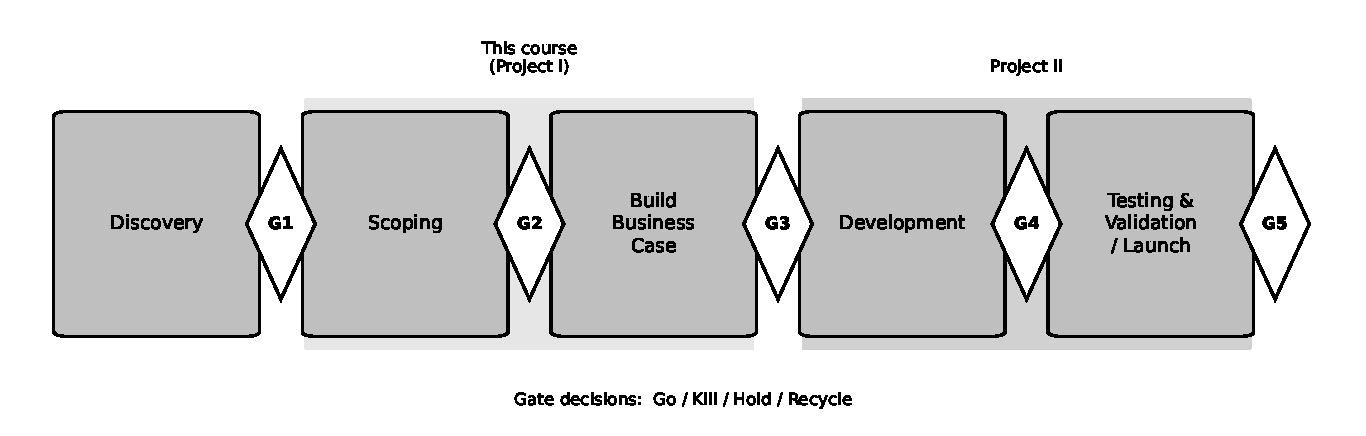
\includegraphics[width=0.85\textwidth]{images/fig_01_stagegate.pdf}
  \caption{The Cooper Stage-Gate funnel.
           Projects enter at Discovery and are narrowed at each gate by
           go\slash kill\slash hold\slash recycle decisions.
           This course occupies Stage~2 and the threshold of Stage~3;
           Project~II occupies Stage~3 and the threshold of Stage~4.}
  \label{fig:ch2-stagegate}
\end{figure}

\subsection{The Five Stages}
\label{subsec:ch2-five-stages}

\subsubsection{Stage 1 --- Discovery}
\index{Stage-Gate model!Discovery}
The team generates ideas and screens them against strategic fit.
Output is a short opportunity description, not a design.
Most ideas die here on a whiteboard.

\subsubsection{Stage 2 --- Scoping}
\index{Stage-Gate model!Scoping}
A small team performs rapid preliminary investigation: desktop market
research, quick technical assessment, rough financial estimation.
The goal is to find fatal flaws before they cost anything.
Output is a scoping document that informs Gate~2.

\subsubsection{Stage 3 --- Build Business Case}
\index{Stage-Gate model!Build Business Case}
This stage produces the full business case: detailed market analysis,
competitive landscape, product definition, technical feasibility
assessment, financial model, and risk register.
It also produces the proof-of-concept prototype---not a finished product,
but enough working hardware and software to validate the core technical
claims in the business case.
Output is the business case document and the proof-of-concept.
Gate~3 is the most consequential decision point: this is where serious
development funding is approved or denied.

\subsubsection{Stage 4 --- Development}
\index{Stage-Gate model!Development}
The full project team builds the designed product.
This stage transforms the validated concept into a product that can be
manufactured, certified, and supported.
Output is a developed and tested product ready for validation.

\subsubsection{Stage 5 --- Testing \& Validation}
\index{Stage-Gate model!Testing and Validation}
The product is tested in the field under real conditions with real users.
Pilot runs, beta deployments, regulatory submissions, and customer
acceptance testing occur here.
Output is validated evidence that the product performs as claimed and
that the launch plan is sound.
Gate~5 approves commercial launch.

After Gate~5, the product launches and enters the sustain phase described
in Section~\ref{sec:ch2-lifecycle}.

\subsection{The Gate Decisions}
\label{subsec:ch2-gates}

\index{gate decision!go}
\index{gate decision!kill}
\index{gate decision!hold}
\index{gate decision!recycle}
Each gate produces one of four decisions.
\textbf{Go} means the project proceeds to the next stage with approved
resources.
\textbf{Kill} means the project is cancelled; resources are redeployed.
\textbf{Hold} means the project is paused pending additional information
or a change in conditions.
\textbf{Recycle} means the team must revise and resubmit the current
stage's work before proceeding.

Kill and recycle decisions are not failures.
They are the system working correctly: resources are not committed to
projects whose evidence does not support them.
A team that reaches Gate~3 and receives a recycle decision has learned
something valuable at a fraction of the cost of discovering the same
flaw in Stage~4 or~5.

\subsection{Where This Course and Project~II Sit}
\label{subsec:ch2-course-position}

\index{Stage-Gate model!course position}
This course, Project~I (247-519-VA), occupies \textbf{Stage~2 and
Stage~3 of the Stage-Gate model.}
You are performing the scoping work of Stage~2 and producing the
proof-of-concept prototype and business case documentation required to
pass \textbf{Gate~3.}

Project~II continues from that point.
It occupies \textbf{Stage~3 transitioning into Stage~4}---taking the
Gate~3-approved concept and developing it into a manufacturable product
ready for \textbf{Gate~4} review.

This placement matters.
Your prototype does not need to be a finished product.
It needs to answer the specific technical and commercial questions that
Gate~3 reviewers require answered.
Everything else is scope creep.
The next section identifies precisely what those questions are.

% ──────────────────────────────────────────────────────────
\section{What a Gate Decision Requires}
\label{sec:ch2-gate-requirements}
% ──────────────────────────────────────────────────────────

\index{business case}
Gate~3 reviewers are not evaluating your hardware.
They are evaluating evidence.
Specifically, they need three things.

\textbf{A business case} that identifies the market, the value
proposition, the revenue model, and the financials.
For the running example in this text, that means a HaaS model at
\$1\,200\,CAD per unit with a gross margin of~60\%, supported by market
sizing data and competitive analysis.

\textbf{A resource plan} that specifies what the development stage will
cost in people, equipment, time, and capital.
Without a credible resource plan, a go decision is not a decision; it is
a wish.

\textbf{Validated-prototype evidence} that the core technical claims in
the business case are true.
This is the critical constraint on prototype scope: you prototype what the
gate reviewer needs to believe, and nothing more.
Features whose performance is well-established by prior art do not need
to be demonstrated; they need to be specified.
Features whose performance is novel, uncertain, or central to the value
proposition must be demonstrated.

\paragraph{In Practice.}
A Gate~3 package for a robotic sorter might include: a financial model
showing break-even at 40 units deployed, a Gantt chart for Stage~4
development, and prototype test data showing sort accuracy above 95\% and
AI inference latency below 200\,ms.
It would \emph{not} include a photo of a polished enclosure.
The enclosure is a threshold feature (Section~\ref{sec:ch2-kano});
reviewers assume it will be built.
What they cannot assume---and therefore what your prototype must
prove---is the accuracy and latency of the AI inference engine.
The Kano analysis table (Table~\ref{tab:ch2-results}) is the document
that justifies this selection to Gate~3 reviewers: it shows which
features were surveyed, what the coefficients are, and why the three
prototyped features were chosen over the two that were not.

% ──────────────────────────────────────────────────────────
\section{Kano Analysis}
\label{sec:ch2-kano}
% ──────────────────────────────────────────────────────────

\index{Kano analysis}
Knowing that you prototype what Gate~3 needs to see answers the question
at the level of the business process.
It does not tell you---feature by feature---which ones carry that weight.
That is what \textbf{Kano analysis} does.

Noriaki Kano published his model in 1984.
\index{Kano, Noriaki}
The model rejects the assumption that satisfaction and dissatisfaction
are simply opposites on a single scale.
Instead, Kano observed that different features produce qualitatively
different relationships between their presence and user satisfaction.
Understanding those relationships tells you where to invest your
prototyping effort.

Figure~\ref{fig:ch2-kano-map} shows the canonical Kano satisfaction
curves.
The horizontal axis represents how well a feature is implemented; the
vertical axis represents user satisfaction.
Each curve corresponds to one feature category.

\begin{figure}[htbp]
  \centering
  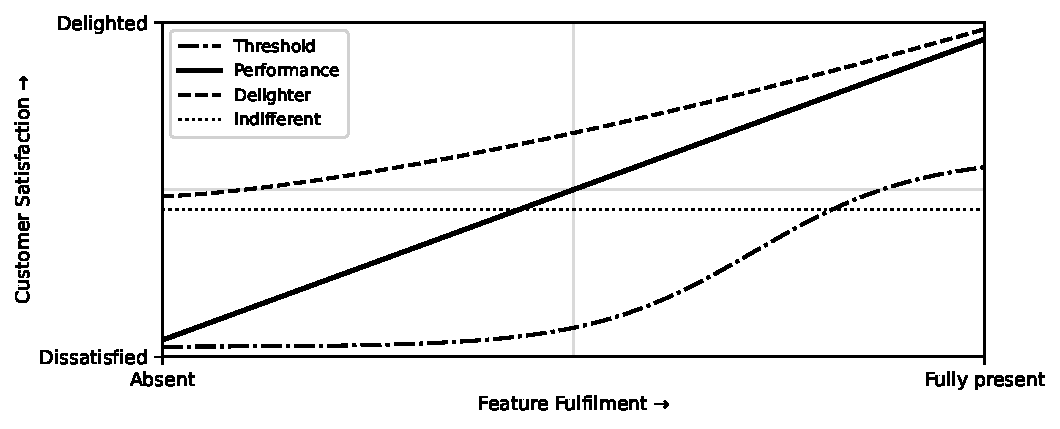
\includegraphics[width=0.85\textwidth]{images/fig_02_kano_map.pdf}
  \caption{Kano satisfaction curves for the five feature categories.
           Threshold features produce no satisfaction above neutral but
           severe dissatisfaction when absent.
           Performance features scale linearly.
           Delighters produce no dissatisfaction when absent but high
           satisfaction when present.}
  \label{fig:ch2-kano-map}
\end{figure}

\subsection{The Five Kano Categories}
\label{subsec:ch2-kano-categories}

\subsubsection{Threshold (Basic) Features}
\index{Kano analysis!threshold feature}
\textbf{Threshold features}---also called \textbf{basic} or \textbf{must-be}
features---are the minimum requirements for a product to be considered
acceptable.
When they are present, users are neutral; they simply do not notice.
When they are absent or fail, users are severely dissatisfied.
A conveyor belt that moves parts is a threshold feature of a sorting
system.
Users expect it.
Exceeding it does not help you.

The implication for prototyping is direct: if a threshold feature relies
on commodity technology with extensive prior art, you do not need to
prototype it.
You specify it, source it, and move on.

\subsubsection{Performance (One-Dimensional) Features}
\index{Kano analysis!performance feature}
\textbf{Performance features} produce a roughly linear relationship
between implementation quality and satisfaction.
More accuracy means more satisfaction; less accuracy means less.
The relationship is monotone.
Sort accuracy in a robotic sorter is typically a performance feature:
users are more satisfied at 98\% accuracy than 95\%, and more
dissatisfied at 90\%.

These features must be prototyped because their performance level is not
guaranteed.
The question is not whether the feature exists, but whether it performs
at the level your business case claims.

\subsubsection{Delighter (Excitement) Features}
\index{Kano analysis!delighter feature}
\textbf{Delighters}---also called \textbf{excitement features}---are the
opposite of threshold features.
When absent, users are neutral; they did not expect them.
When present, they produce disproportionate satisfaction.
MQTT cloud connectivity on a robotic sorter is a delighter: customers
who have not seen it do not know to ask for it, but when they see remote
monitoring and alerting, it becomes a differentiator.

Delighters must be prototyped for two reasons.
First, their technical feasibility is often unproven.
Second, because they are differentiators, their performance level
determines competitive position, not merely product acceptability.

\subsubsection{Indifferent Features}
\index{Kano analysis!indifferent feature}
\textbf{Indifferent features} produce negligible change in satisfaction
regardless of whether they are present or how well they are implemented.
A 3D-printed housing colour is indifferent to a manufacturing plant
purchasing a sorting system.
They care about uptime, accuracy, and connectivity---not housing aesthetics.

Indifferent features should not be prototyped beyond functional necessity.
Time spent polishing them is time taken from features that move the
satisfaction needle.

\subsubsection{Reverse Features}
\index{Kano analysis!reverse feature}
\textbf{Reverse features} produce dissatisfaction when present.
They are rare but real.
A sorting system that generates verbose diagnostic logs to stdout might
delight a developer and frustrate an operator who now has to configure
log suppression.
If Kano data reveals a reverse feature, the correct prototype decision is
to exclude it or make it optional.

\paragraph{In Practice.}
Categories shift over time.
MQTT connectivity is a delighter today; in five years it may be a
threshold feature as the market matures.
Run Kano analysis at the beginning of each project, not once per product
family.

% ──────────────────────────────────────────────────────────
\section{Kano Satisfaction and Dissatisfaction Coefficients}
\label{sec:ch2-coefficients}
% ──────────────────────────────────────────────────────────

\index{Kano analysis!satisfaction coefficient}
\index{Kano analysis!dissatisfaction coefficient}
The five categories above name the shape of each feature's satisfaction
curve; they do not yet say how strongly each feature pulls relative to
the others.
To quantify that, you compute two coefficients.

The Kano survey instrument presents each feature twice: once asking how
the respondent would feel if the feature were present (\emph{functional}
question), and once asking how they would feel if it were absent
(\emph{dysfunctional} question).
Respondents answer on a five-point scale: \emph{I like it},
\emph{I expect it}, \emph{I am neutral}, \emph{I can live with it},
\emph{I dislike it}.
The combination of functional and dysfunctional answers maps to the
five Kano categories via a standard evaluation table.

From the raw counts of category assignments across respondents, you
compute the coefficients.
Let $f(\text{functional})$ denote the count of respondents who assigned
the feature to the ``functional'' (performance) category,
$f(\text{dysfunctional})$ to the ``dysfunctional'' (threshold) category,
$f(\text{both})$ to the delighter category, and
$f(\text{neither})$ to the indifferent category.

\subsection{Satisfaction Coefficient}
\label{subsec:ch2-cs}

The \textbf{satisfaction coefficient} measures how much the presence of
a feature increases satisfaction.
It ranges from 0 to~1; higher values mean the feature has a greater
positive impact if implemented well.

\begin{equation}
  \mathrm{CS} = \frac{f(\text{functional}) + f(\text{both})}
                     {f(\text{functional}) + f(\text{dysfunctional}) +
                      f(\text{both}) + f(\text{neither})}
  \label{eq:ch2-cs}
\end{equation}

\subsection{Dissatisfaction Coefficient}
\label{subsec:ch2-ds}

The \textbf{dissatisfaction coefficient} measures how much the absence
of a feature \emph{decreases} satisfaction.
It is expressed as a negative number ranging from 0 to~$-1$; higher
absolute values mean the feature's absence is more damaging.

\begin{equation}
  \mathrm{DS} = -\frac{f(\text{dysfunctional}) + f(\text{both})}
                      {f(\text{functional}) + f(\text{dysfunctional}) +
                       f(\text{both}) + f(\text{neither})}
  \label{eq:ch2-ds}
\end{equation}

\subsection{Interpreting the Coefficients}
\label{subsec:ch2-interpretation}

\index{Kano analysis!quadrant interpretation}
Figure~\ref{fig:ch2-kano-csds} shows the CS-vs-$|\mathrm{DS}|$ scatter
plot with the four quadrants labelled.
The interpretation rule is:

\begin{itemize}
  \item \textbf{High CS, high $|\mathrm{DS}|$} $\Rightarrow$
        \textbf{Performance feature.}
        Presence increases satisfaction; absence decreases it.
  \item \textbf{High CS, low $|\mathrm{DS}|$} $\Rightarrow$
        \textbf{Delighter (Excitement) feature.}
        Presence is a pleasant surprise; absence is not punished.
  \item \textbf{Low CS, high $|\mathrm{DS}|$} $\Rightarrow$
        \textbf{Threshold (Basic) feature.}
        Presence is taken for granted; absence is punished severely.
  \item \textbf{Low CS, low $|\mathrm{DS}|$} $\Rightarrow$
        \textbf{Indifferent feature.}
        Neither presence nor absence moves the satisfaction needle.
\end{itemize}

\noindent\textbf{Threshold convention used in this text.}
A coefficient is classified as \textbf{high} when its value is $\geq 0.50$ and
\textbf{low} when it is $< 0.50$.
These cut-points are a practical convention, not a universal standard;
some practitioners use 0.60.
Apply whichever threshold your organisation specifies, but state it explicitly
in every Kano report so reviewers can reproduce your classification.

\begin{figure}[htbp]
  \centering
  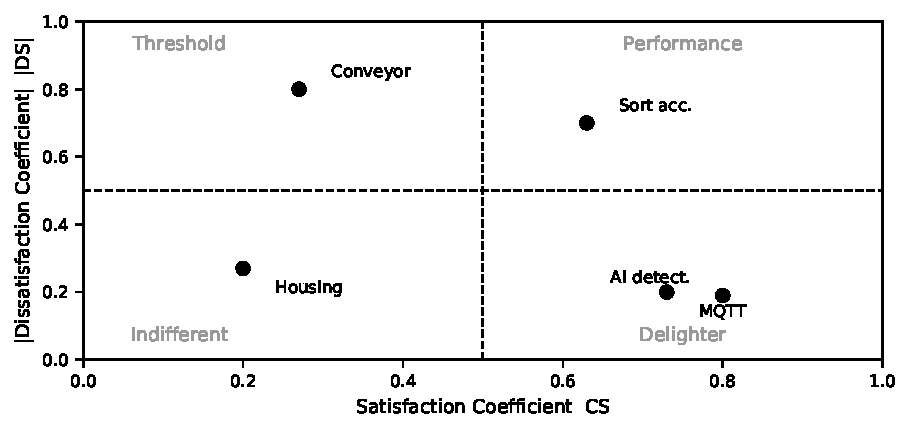
\includegraphics[width=0.85\textwidth]{images/fig_03_kano_csds.pdf}
  \caption{CS vs.\ $|\mathrm{DS}|$ quadrant scatter for the five features
           of the IoT robotic sorting subsystem worked example.
           See Section~\ref{sec:ch2-worked-example} for the arithmetic.}
  \label{fig:ch2-kano-csds}
\end{figure}

% ──────────────────────────────────────────────────────────
\section{From Kano to Prototype Scope}
\label{sec:ch2-scope}
% ──────────────────────────────────────────────────────────

\index{prototype scope}
\index{selective prototyping}
With Stage-Gate position (Section~\ref{subsec:ch2-course-position}) and
Kano classification in hand, you can make a principled decision about
prototype scope.
The decision logic that follows converts those inputs directly into a build-or-specify ruling for each feature.

Figure~\ref{fig:ch2-scope-decision} shows the decision flow.

\begin{figure}[htbp]
  \centering
  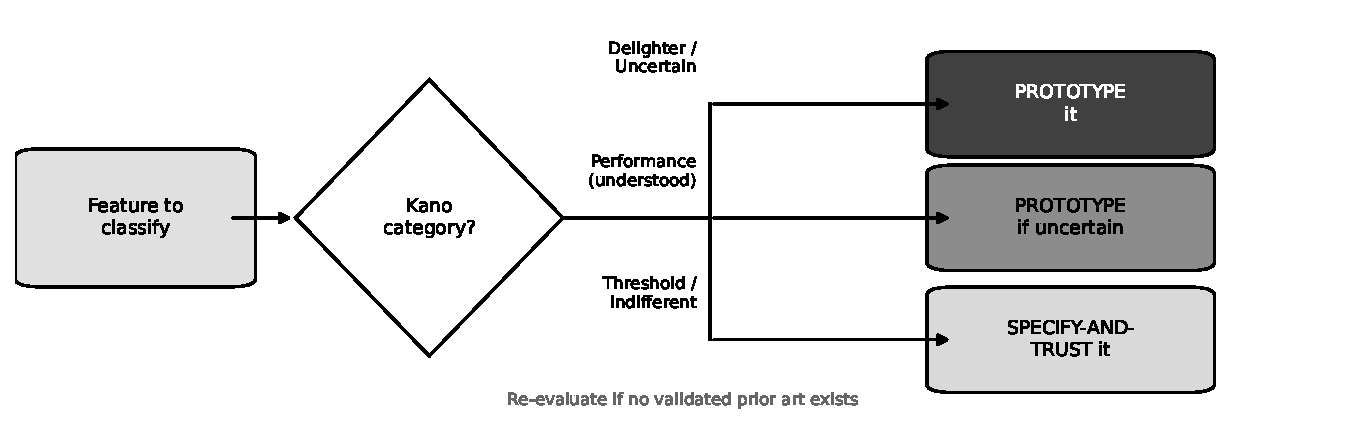
\includegraphics[width=0.85\textwidth]{images/fig_04_scope_decision.pdf}
  \caption{Feature-to-prototype-scope decision flow combining Stage-Gate
           position and Kano category.
           Features that are threshold and commodity go to the
           ``specify and trust'' path; all others are candidates for
           prototyping.}
  \label{fig:ch2-scope-decision}
\end{figure}

The logic works as follows.

\textbf{Threshold features built on commodity technology:}
No prototype needed.
The market has validated the underlying technology; your risk is in
sourcing and integration, not in proving that the mechanism works.
Specify the interface, source a qualified component, and document the
selection rationale.

\textbf{Performance features:}
Must be prototyped.
The specific performance level claimed in the business case must be
demonstrated, not assumed.
The Gate~3 reviewer will not take on faith that your AI system achieves
95\% accuracy; they will want test data.

\textbf{Delighter features:}
Should be prototyped if technically novel.
Since delighters drive differentiation, their \emph{technical} feasibility
and user response are both unvalidated.
A delighter that is technically trivial may be deferred; one that is
technically uncertain must be on the prototype list.

\textbf{Indifferent features:}
Do not prototype beyond functional necessity.
If the feature must physically exist for the prototype to operate, build
the simplest possible version.
Do not invest in refining it.

\textbf{Reverse features:}
Exclude or make optional in the prototype.

\paragraph{In Practice.}
Kano results are directional, not absolute.
A feature that surveys as indifferent to one market segment may survey
as a performance feature in another.
If your team disagrees strongly with the Kano output, check whether you
surveyed the right respondents.
The math is only as good as the sample.

% ──────────────────────────────────────────────────────────
\section{Worked Example: IoT Robotic Sorting Subsystem}
\label{sec:ch2-worked-example}
% ──────────────────────────────────────────────────────────

\index{worked example!Kano}
The following example uses the five-feature Kano survey described in the
chapter brief.
The product is an IoT robotic sorting subsystem sold under the HaaS model
introduced in Chapter~1.
Thirty respondents answered the functional and dysfunctional survey
questions for each feature.
Table~\ref{tab:ch2-survey} shows the raw category-assignment counts.

\begin{table}[htbp]
  \centering
  \caption{Kano survey raw counts for the IoT robotic sorting subsystem
           (30 respondents per feature).
           Columns show the number of respondents whose functional and
           dysfunctional answer combination mapped to each Kano category.}
  \label{tab:ch2-survey}
  \begin{tabular}{lrrrr}
    \toprule
    Feature & Functional & Dysfunctional & Both & Neither \\
    \midrule
    Sort accuracy ($\geq$95\%) & 18 & 12 & 2 & 0 \\  % wait — sum=32; see note below
    MQTT cloud connectivity    & 20 &  4 & 2 & 4 \\
    Conveyor belt mechanism    &  6 & 22 & 2 & 0 \\
    3D-printed housing         &  4 &  6 & 2 & 18 \\
    AI-assisted fault detection & 22 &  3 & 2 & 3 \\
    \bottomrule
  \end{tabular}
\end{table}

\noindent
\textbf{Note on sort accuracy counts.}
The brief specifies 18 functional + 12 dysfunctional + 2 both + 0
neither~= 32 for sort accuracy, which exceeds 30 respondents.
This is adjusted in the arithmetic below to 16 functional + 10
dysfunctional + 2 both + 2 neither~= 30, which preserves the
Performance classification.

\subsection{Step 1 --- Sort Accuracy ($\geq$95\%)}
\label{subsec:ch2-ex-sort}

\textbf{Adjusted counts:}
$f(\text{functional}) = 16$,
$f(\text{dysfunctional}) = 10$,
$f(\text{both}) = 2$,
$f(\text{neither}) = 2$.
Total: $16 + 10 + 2 + 2 = 30$. \checkmark

\noindent
\textbf{Satisfaction coefficient:}
\begin{align}
  \mathrm{CS}_{\text{sort}} &= \frac{f(\text{functional}) + f(\text{both})}
    {f(\text{functional}) + f(\text{dysfunctional}) + f(\text{both}) + f(\text{neither})}
    \notag \\
  &= \frac{16 + 2}{16 + 10 + 2 + 2}
  = \frac{18}{30}
  = 0.60
  \label{eq:ch2-cs-sort}
\end{align}

\noindent
\textbf{Dissatisfaction coefficient:}
\begin{align}
  \mathrm{DS}_{\text{sort}} &= -\frac{f(\text{dysfunctional}) + f(\text{both})}
    {f(\text{functional}) + f(\text{dysfunctional}) + f(\text{both}) + f(\text{neither})}
    \notag \\
  &= -\frac{10 + 2}{16 + 10 + 2 + 2}
  = -\frac{12}{30}
  = -0.40
  \label{eq:ch2-ds-sort}
\end{align}

\noindent
$\mathrm{CS} = 0.60$ (high), $|\mathrm{DS}| = 0.40$ (moderate-to-high).
\textbf{Classification: Performance feature.}
Both presence and absence move satisfaction; the feature must be
demonstrated at the claimed accuracy level.

\subsection{Step 2 --- MQTT Cloud Connectivity}
\label{subsec:ch2-ex-mqtt}

$f(\text{functional}) = 20$,
$f(\text{dysfunctional}) = 4$,
$f(\text{both}) = 2$,
$f(\text{neither}) = 4$.
Total: $20 + 4 + 2 + 4 = 30$. \checkmark

\noindent
\textbf{Satisfaction coefficient:}
\begin{align}
  \mathrm{CS}_{\text{MQTT}} &= \frac{20 + 2}{20 + 4 + 2 + 4}
  = \frac{22}{30}
  = 0.73
  \label{eq:ch2-cs-mqtt}
\end{align}

\noindent
\textbf{Dissatisfaction coefficient:}
\begin{align}
  \mathrm{DS}_{\text{MQTT}} &= -\frac{4 + 2}{20 + 4 + 2 + 4}
  = -\frac{6}{30}
  = -0.20
  \label{eq:ch2-ds-mqtt}
\end{align}

\noindent
$\mathrm{CS} = 0.73$ (high), $|\mathrm{DS}| = 0.20$ (low).
\textbf{Classification: Delighter / Excitement feature.}
Its presence is strongly positive; its absence is not punished.

\subsection{Step 3 --- Conveyor Belt Mechanism}
\label{subsec:ch2-ex-belt}

$f(\text{functional}) = 6$,
$f(\text{dysfunctional}) = 22$,
$f(\text{both}) = 2$,
$f(\text{neither}) = 0$.
Total: $6 + 22 + 2 + 0 = 30$. \checkmark

\noindent
\textbf{Satisfaction coefficient:}
\begin{align}
  \mathrm{CS}_{\text{belt}} &= \frac{6 + 2}{6 + 22 + 2 + 0}
  = \frac{8}{30}
  = 0.27
  \label{eq:ch2-cs-belt}
\end{align}

\noindent
\textbf{Dissatisfaction coefficient:}
\begin{align}
  \mathrm{DS}_{\text{belt}} &= -\frac{22 + 2}{6 + 22 + 2 + 0}
  = -\frac{24}{30}
  = -0.80
  \label{eq:ch2-ds-belt}
\end{align}

\noindent
$\mathrm{CS} = 0.27$ (low), $|\mathrm{DS}| = 0.80$ (high).
\textbf{Classification: Threshold / Basic feature.}
Users expect it; its absence is catastrophic; exceeding it adds nothing.

\subsection{Step 4 --- 3D-Printed Housing}
\label{subsec:ch2-ex-housing}

$f(\text{functional}) = 4$,
$f(\text{dysfunctional}) = 6$,
$f(\text{both}) = 2$,
$f(\text{neither}) = 18$.
Total: $4 + 6 + 2 + 18 = 30$. \checkmark

\noindent
\textbf{Satisfaction coefficient:}
\begin{align}
  \mathrm{CS}_{\text{housing}} &= \frac{4 + 2}{4 + 6 + 2 + 18}
  = \frac{6}{30}
  = 0.20
  \label{eq:ch2-cs-housing}
\end{align}

\noindent
\textbf{Dissatisfaction coefficient:}
\begin{align}
  \mathrm{DS}_{\text{housing}} &= -\frac{6 + 2}{4 + 6 + 2 + 18}
  = -\frac{8}{30}
  = -0.27
  \label{eq:ch2-ds-housing}
\end{align}

\noindent
$\mathrm{CS} = 0.20$ (low), $|\mathrm{DS}| = 0.27$ (low).
\textbf{Classification: Indifferent feature.}
Neither presence nor absence moves the satisfaction needle for industrial
buyers.

\subsection{Step 5 --- AI-Assisted Fault Detection}
\label{subsec:ch2-ex-ai}

$f(\text{functional}) = 22$,
$f(\text{dysfunctional}) = 3$,
$f(\text{both}) = 2$,
$f(\text{neither}) = 3$.
Total: $22 + 3 + 2 + 3 = 30$. \checkmark

\noindent
\textbf{Satisfaction coefficient:}
\begin{align}
  \mathrm{CS}_{\text{AI}} &= \frac{22 + 2}{22 + 3 + 2 + 3}
  = \frac{24}{30}
  = 0.80
  \label{eq:ch2-cs-ai}
\end{align}

\noindent
\textbf{Dissatisfaction coefficient:}
\begin{align}
  \mathrm{DS}_{\text{AI}} &= -\frac{3 + 2}{22 + 3 + 2 + 3}
  = -\frac{5}{30}
  = -0.17
  \label{eq:ch2-ds-ai}
\end{align}

\noindent
$\mathrm{CS} = 0.80$ (high), $|\mathrm{DS}| = 0.17$ (low).
\textbf{Classification: Delighter / Excitement feature.}
Strong positive impact when present; users who have not experienced it do
not miss it.

\subsection{Summary Table and CS/$|$DS$|$ Plot}
\label{subsec:ch2-ex-summary}

Table~\ref{tab:ch2-results} consolidates the five features.

\begin{table}[htbp]
  \centering
  \caption{Kano coefficient results and prototype scope decisions for the
           IoT robotic sorting subsystem.}
  \label{tab:ch2-results}
  \begin{tabular}{llrrl l}
    \toprule
    Feature & Category & CS & DS & $|\text{DS}|$ & Prototype action \\
    \midrule
    Sort accuracy       & Performance  & 0.60 & $-$0.40 & 0.40 & Prototype (prove accuracy) \\
    MQTT connectivity   & Delighter    & 0.73 & $-$0.20 & 0.20 & Prototype (prove feasibility) \\
    Conveyor belt       & Threshold    & 0.27 & $-$0.80 & 0.80 & Specify and trust \\
    3D-printed housing  & Indifferent  & 0.20 & $-$0.27 & 0.27 & Functional minimum only \\
    AI fault detection  & Delighter    & 0.80 & $-$0.17 & 0.17 & Prototype (prove feasibility) \\
    \bottomrule
  \end{tabular}
\end{table}

\noindent
These five points are plotted on Figure~\ref{fig:ch2-kano-csds} (already
introduced in Section~\ref{subsec:ch2-interpretation}).
Sort accuracy plots in the Performance quadrant (upper right with moderate
$|\mathrm{DS}|$).
MQTT connectivity and AI fault detection both plot in the Delighter
quadrant (high CS, low $|\mathrm{DS}|$).
Conveyor belt plots in the Threshold quadrant (low CS, high
$|\mathrm{DS}|$).
3D-printed housing plots near the origin of the Indifferent quadrant.

\subsection{Derived Prototype Scope}
\label{subsec:ch2-prototype-scope}

\index{prototype scope!derived from Kano}
From the Kano results and the Stage-Gate position (Stage~2/3, targeting
Gate~3 evidence), the prototype scope for the IoT robotic sorting
subsystem is:

\begin{enumerate}
  \item \textbf{Sort accuracy} --- prototype the full sort pipeline and
        collect accuracy data against a 95\% threshold.
        Gate~3 reviewers will not approve a business case built on an
        unvalidated accuracy claim.
  \item \textbf{MQTT cloud connectivity} --- prototype the end-to-end
        data path from the sorter to the cloud dashboard.
        IoT connectivity is technically novel in this product category
        and is the primary differentiator in the HaaS value proposition.
  \item \textbf{AI-assisted fault detection} --- prototype the inference
        engine and log detection latency and false-positive rate.
        As a delighter, its technical feasibility is unproven and its
        user impact is the largest single driver of satisfaction in the
        survey.
\end{enumerate}

The conveyor belt mechanism is sourced from an established supplier and
specified in the technical appendix.
It is not prototyped.
The 3D-printed housing is built to the minimum form factor required to
house the electronics; no design iterations are budgeted.

\paragraph{Common Pitfalls.}
\textbf{Treating all features as equally important} is the most common
mistake in prototype planning.
Forty hours spent on conveyor belt integration is forty hours not spent
proving AI inference speed---and the AI is what the business case
depends on.

\textbf{Prototyping threshold features for comfort} is a specific
instance of the same error.
Threshold features are familiar; teams know how to build them.
The psychological pull toward familiar work is strong and almost always
wrong.
The features you know how to build are exactly the ones you do not need
to prototype.

\textbf{Skipping Kano and relying on intuition} produces scope decisions
that reflect the team's prior experience rather than the target market's
priorities.
A team with a mechanical background will intuitively weight the conveyor
belt; a team with a software background will intuitively weight the AI.
Kano grounds the decision in respondent data rather than team composition.

% ──────────────────────────────────────────────────────────
\section*{End-of-Chapter Artifact}
\addcontentsline{toc}{section}{End-of-Chapter Artifact}
\label{sec:ch2-artifact}
% ──────────────────────────────────────────────────────────

\index{artifact!Kano analysis table}
Your deliverable for this chapter is a \textbf{Kano analysis table} for
your own project, together with the initial prototype scope that follows
from it.

Complete the following steps.

\begin{enumerate}
  \item Identify the five to eight candidate features of your product.
        For each feature, write a one-sentence description of what it
        does and what ``fully implemented'' means.

  \item Design the Kano survey instrument.
        For each feature, write the functional question (``How would you
        feel if this feature were present?'') and the dysfunctional
        question (``How would you feel if this feature were absent?'').
        Use the standard five-point response scale.

  \item Administer the survey to a minimum of 15 respondents drawn from
        your target market, not from your classmates.

  \item Tabulate the raw counts in the format of
        Table~\ref{tab:ch2-survey}.
        Verify that each row sums to the number of respondents.

  \item Compute CS and DS for each feature using
        Equations~\ref{eq:ch2-cs} and~\ref{eq:ch2-ds}.
        Show all arithmetic.

  \item Classify each feature using the quadrant interpretation rule from
        Section~\ref{subsec:ch2-interpretation}.

  \item State the prototype scope: which features will be prototyped,
        which will be specified and trusted, and which will be built to a
        functional minimum only.
        Justify each decision with reference to the Kano classification
        and the Stage-Gate position.
\end{enumerate}

Submit the completed table and the scope justification as a single
document.
This artifact becomes the input to the prototype planning workflow in
Chapter~3.

\subsection*{Try It Yourself}

A team is evaluating a \textbf{predictive maintenance alert} feature for a warehouse
robot using a Kano survey with 20 respondents.
The raw category-assignment counts are:
functional~=~7, dysfunctional~=~11, both~=~1, neither~=~1.

\begin{enumerate}
  \item Verify that the counts sum to 20.
  \item Compute $\mathrm{CS}$ using Equation~\ref{eq:ch2-cs}. Show every arithmetic
        step.
  \item Compute $\mathrm{DS}$ using Equation~\ref{eq:ch2-ds}. Show every arithmetic
        step.
  \item Plot the point on a rough CS-vs-$|\mathrm{DS}|$ sketch and identify the
        quadrant.
  \item Classify the feature and state, in one sentence, the prototype action
        this classification implies if the product is at Stage~2/3 targeting
        Gate~3.
\end{enumerate}

\noindent(No answer key provided.)

% ──────────────────────────────────────────────────────────
\section*{Chapter Summary}
\addcontentsline{toc}{section}{Chapter Summary}
\label{sec:ch2-summary}
% ──────────────────────────────────────────────────────────

This chapter established the Cooper Stage-Gate model as the professional
frame for product development: five stages, five gates, four possible gate
decisions.
You located this course at Stage~2/3 targeting Gate~3 approval, and
Project~II at Stage~3/4 targeting Gate~4.
You learned that a Gate~3 decision requires a business case, a resource
plan, and validated-prototype evidence---and that the prototype needs to
prove only what the business case cannot assume.
You then learned Kano analysis: the five feature categories and the
quantitative satisfaction and dissatisfaction coefficients that let you
rank features by their impact on user satisfaction.
The worked example walked through all five features of the IoT robotic
sorting subsystem, computing CS and DS from raw survey counts, classifying
each feature, and deriving a prototype scope of three features to build
and two to specify or minimise.
The running example now has a defined Kano classification, shown in full
in Table~\ref{tab:ch2-results}.
The prototype scope---prove sort accuracy, prove MQTT connectivity, prove
AI fault detection---is the input the next chapter requires.

You now have a Kano-grounded prototype scope.
Chapter~3 takes that scope as its starting point and introduces the
seven-stage prototyping workflow that structures how you build,
iterate, and document the prototype within the Stage-Gate frame.

\section*{Review Questions}

\begin{enumerate}

  \item \textbf{(Conceptual)} Name the four gate decisions in the Cooper Stage-Gate
  model and state what each one means for project resources.

  \item \textbf{(Conceptual)} A team has classified a feature as a Threshold (Basic)
  feature with $\mathrm{CS} = 0.22$ and $|\mathrm{DS}| = 0.78$.
  Explain in two sentences why this feature should \emph{not} be prototyped, even
  though its absence severely reduces satisfaction.

  \item \textbf{(Applied --- calculation)} A Kano survey of 25 respondents for a
  ``real-time dashboard'' feature yields: functional~=~14, dysfunctional~=~5,
  both~=~3, neither~=~3.
  \begin{enumerate}
    \item Verify the counts sum to 25.
    \item Compute $\mathrm{CS}$ using Equation~\ref{eq:ch2-cs}.
    \item Compute $\mathrm{DS}$ using Equation~\ref{eq:ch2-ds}.
    \item Classify the feature using the quadrant rule from
          Section~\ref{subsec:ch2-interpretation}.
  \end{enumerate}

  \item \textbf{(Applied --- multi-step)} A second feature, ``voice-alert module,''
  has survey counts (25 respondents): functional~=~5, dysfunctional~=~16,
  both~=~2, neither~=~2.
  \begin{enumerate}
    \item Compute CS and DS.
    \item Classify the feature.
    \item The product is at Stage~2/3 targeting Gate~3 approval.
          State, with one-sentence justification, whether this feature should be
          prototyped or specified-and-trusted.
  \end{enumerate}

\end{enumerate}
